\newpage

\section{Trapezoid Area}

\begin{prob}
In this activity, we explore several ways of justifying the formula for the area of a trapezoid, as labeled below. 
\[
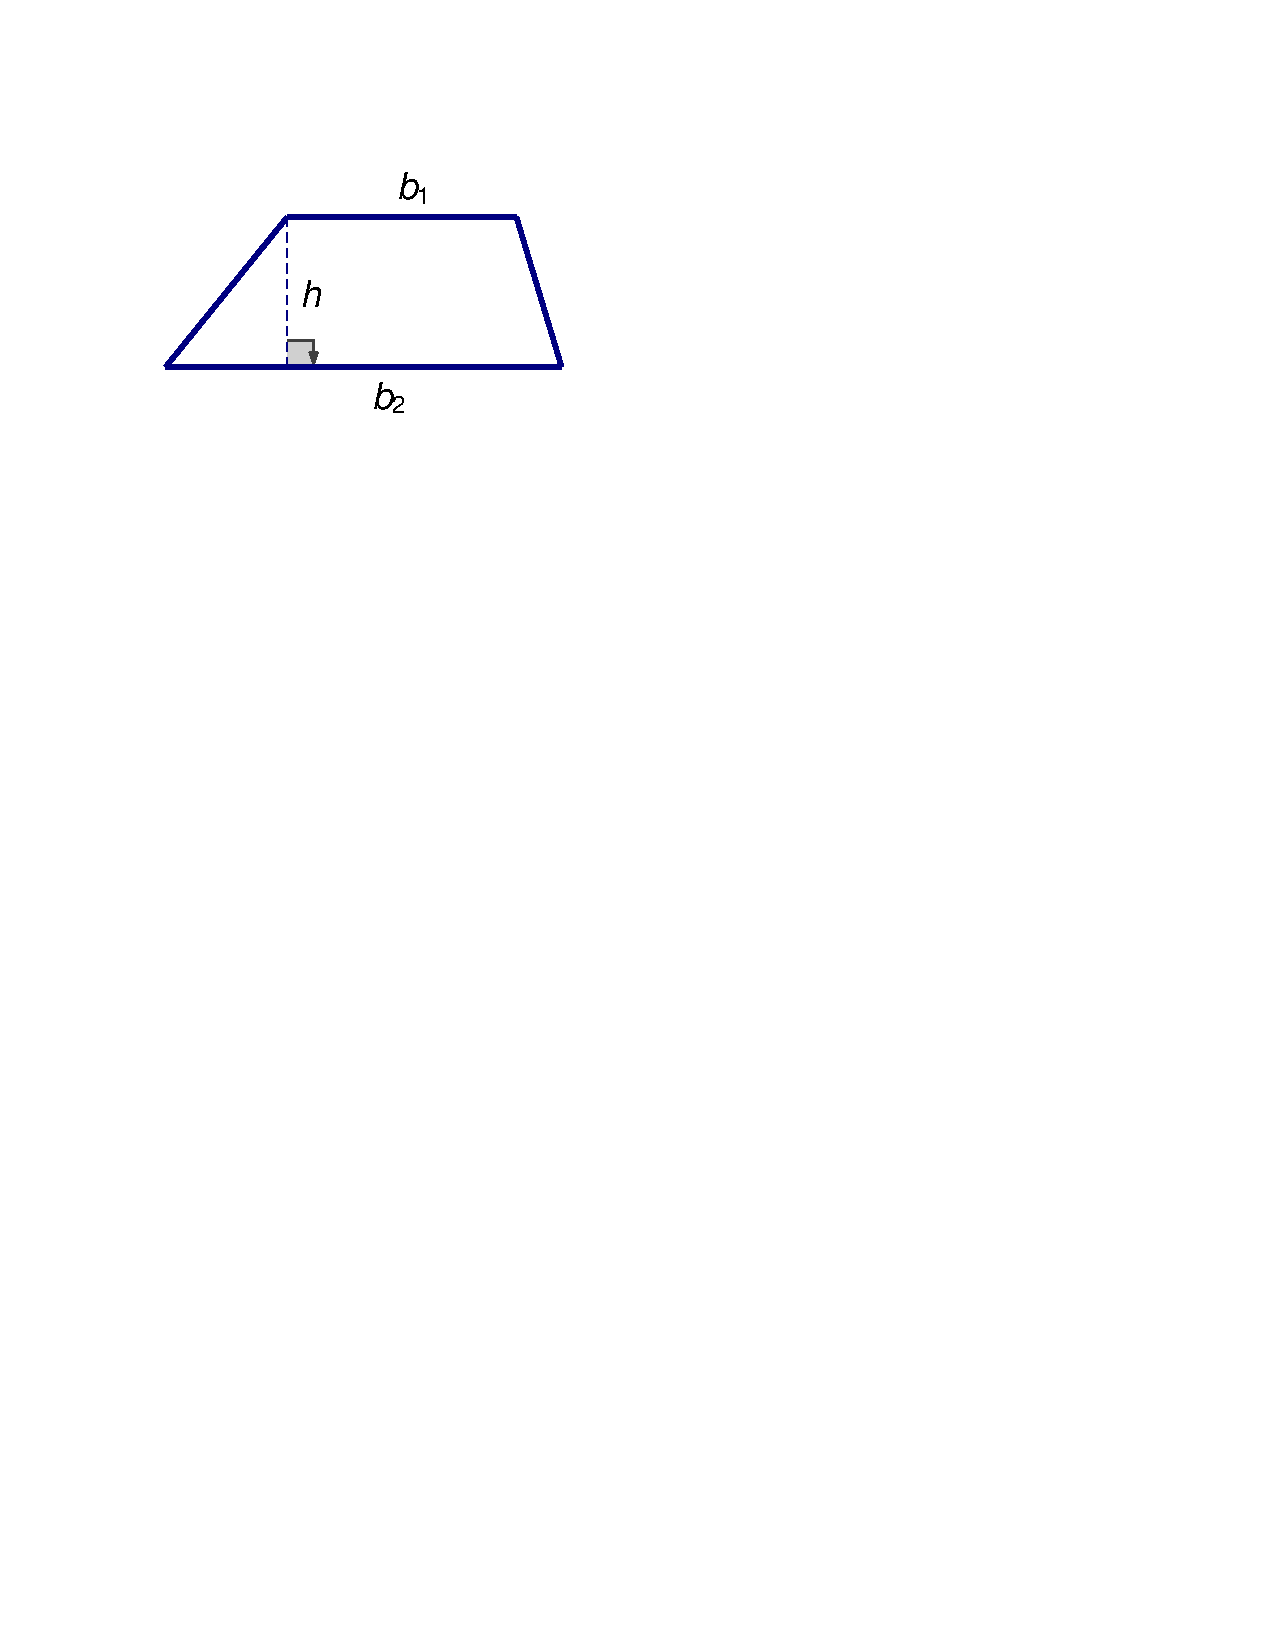
\includegraphics[scale=0.6]{../graphics/trapezoid1.pdf}
\]
Complete the table on the following page so that in each row the explanation, the figure, and the area formula together describe a way of computing the area.  For comparison purposes, each illustration should include a trapezoid congruent to the trapezoid above.   

All of the area formulas will, of course, be equivalent to one another as expressions.  But each way of expressing the area will make the most sense with figure and the explanation from the same row.  

\newpage

\newlength{\formulawidth}
\settowidth{\formulawidth}{$\frac{1}{2}b_2(x+h)-\frac{1}{2}b_1x$, with $\frac{x}{b_1}=\frac{x+h}{b_2}$}  

{\renewcommand{\arraystretch}{1.5}
\begin{tabular}{|>{\centering\arraybackslash}m{2.5cm}|>{\centering\arraybackslash}m{9.5cm}|c|}\hline
Explanation & Figure & Area Formula \\\hline

Rectangle with width that is the average of the bases. & 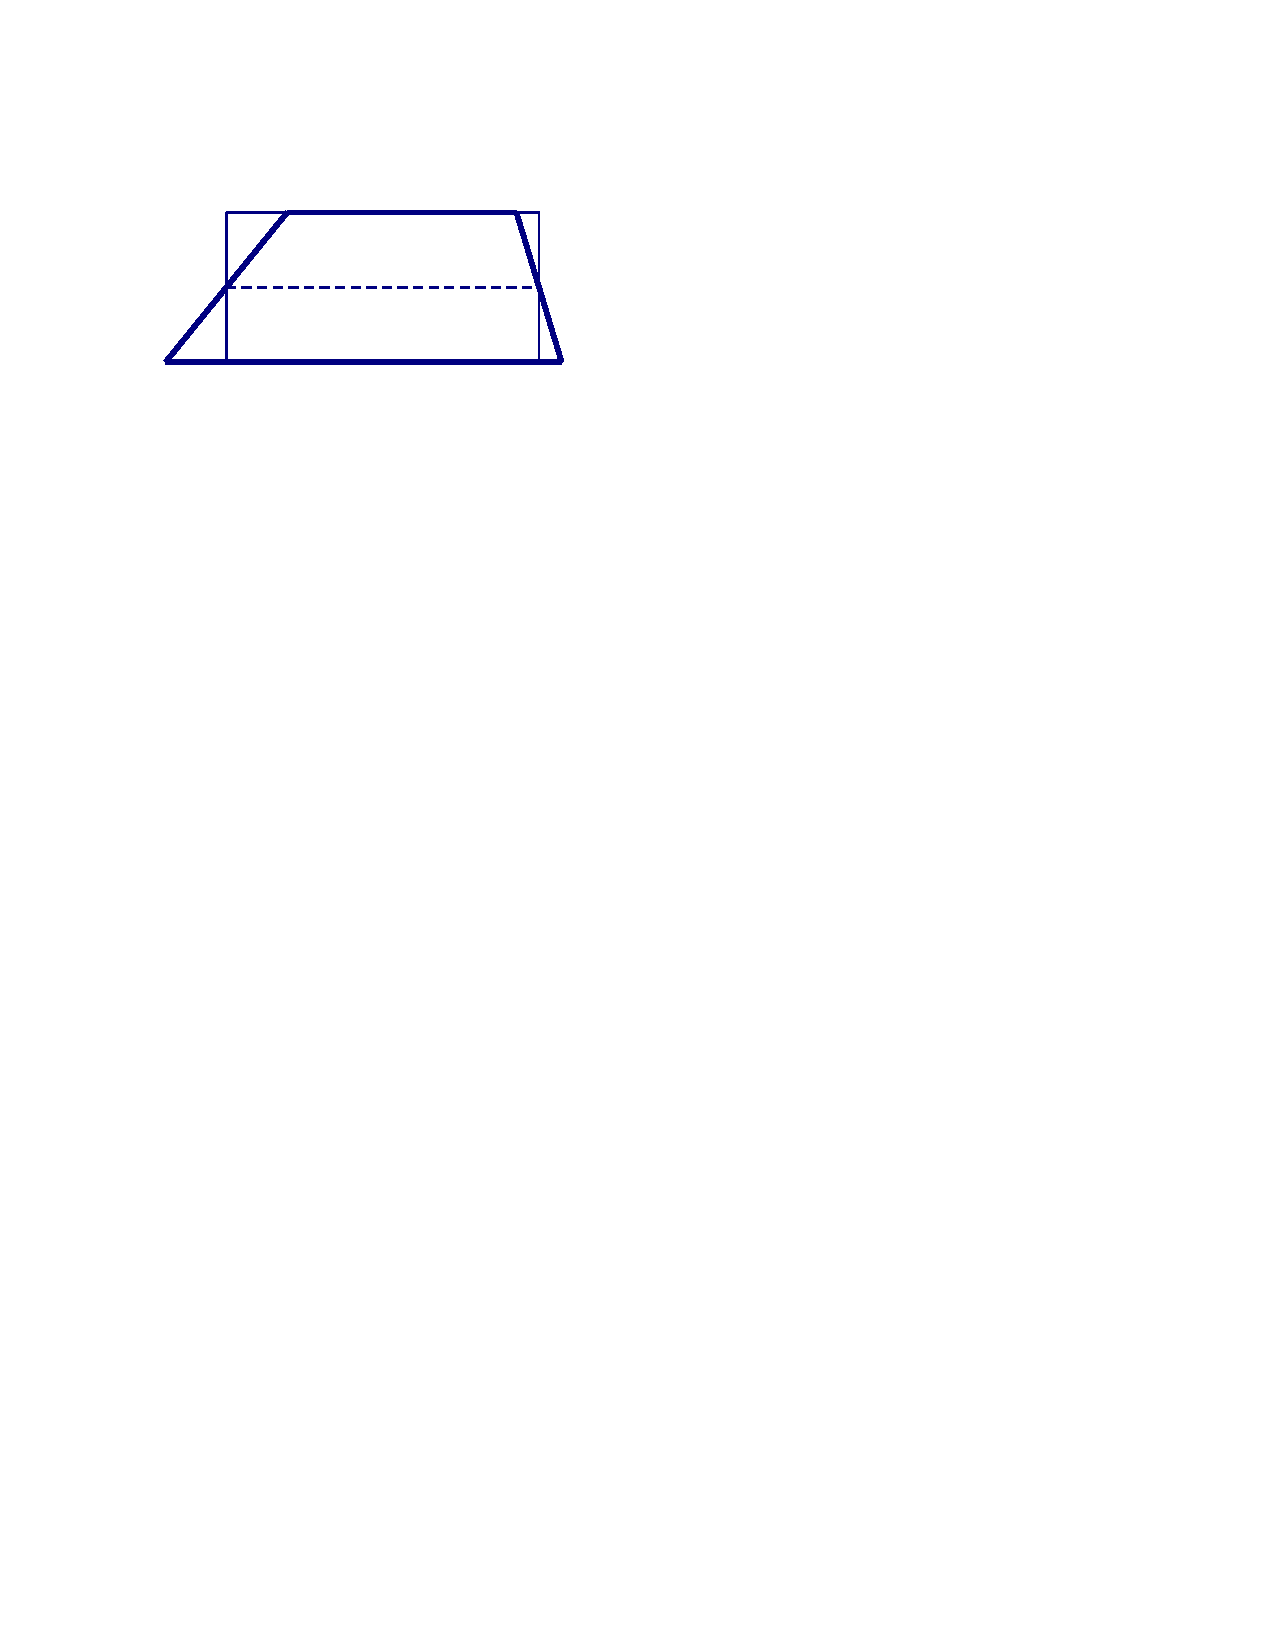
\includegraphics[scale=0.7]{../graphics/trapezoid2.pdf} & $\left(\frac{b_1+b_2}{2}\right)h$ \\ \hline
                              & 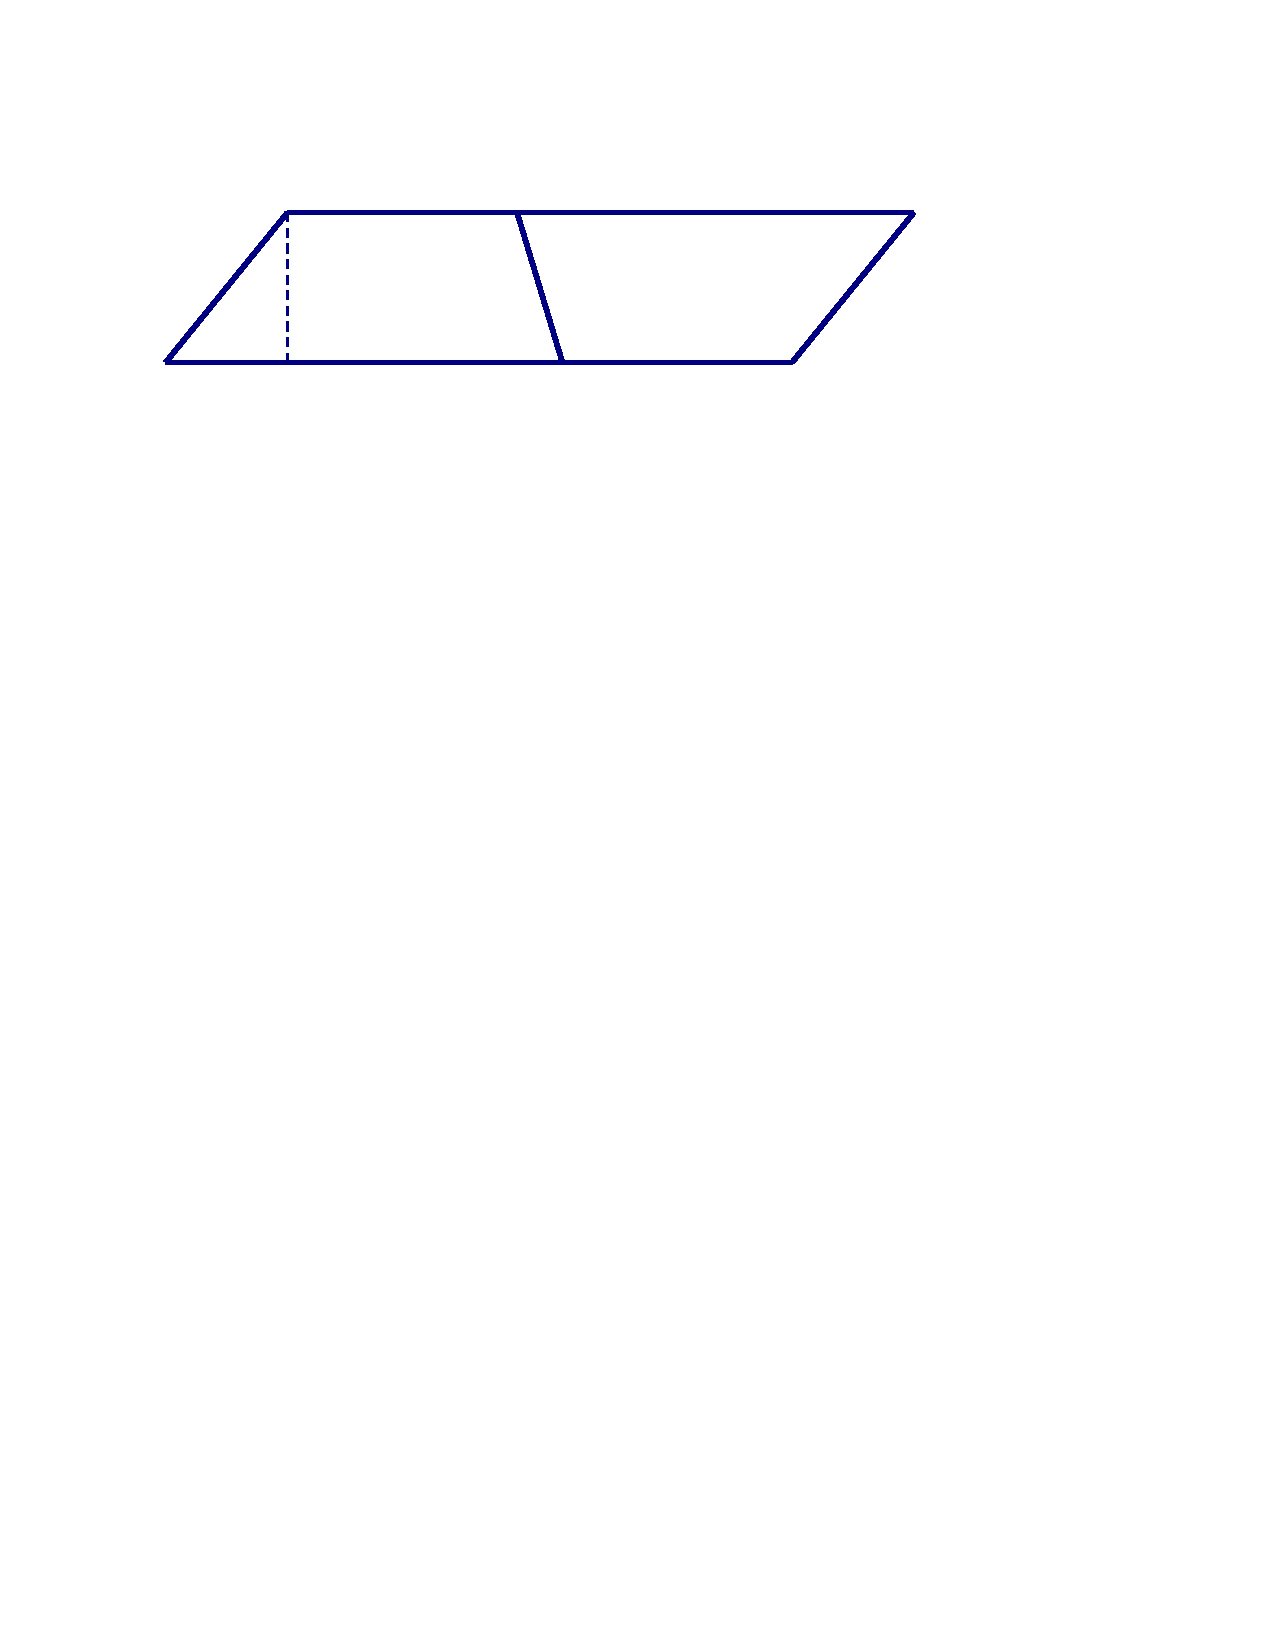
\includegraphics[scale=0.7]{../graphics/trapezoid3.pdf} &                      \\ \hline
Two triangles with the same height and different bases. &                 & \\ \hline
 & & \\ 
\bigskip                              &  & $(b_1+b_2)\frac{h}{2}$ \\ 
 & & \\ \hline
          & 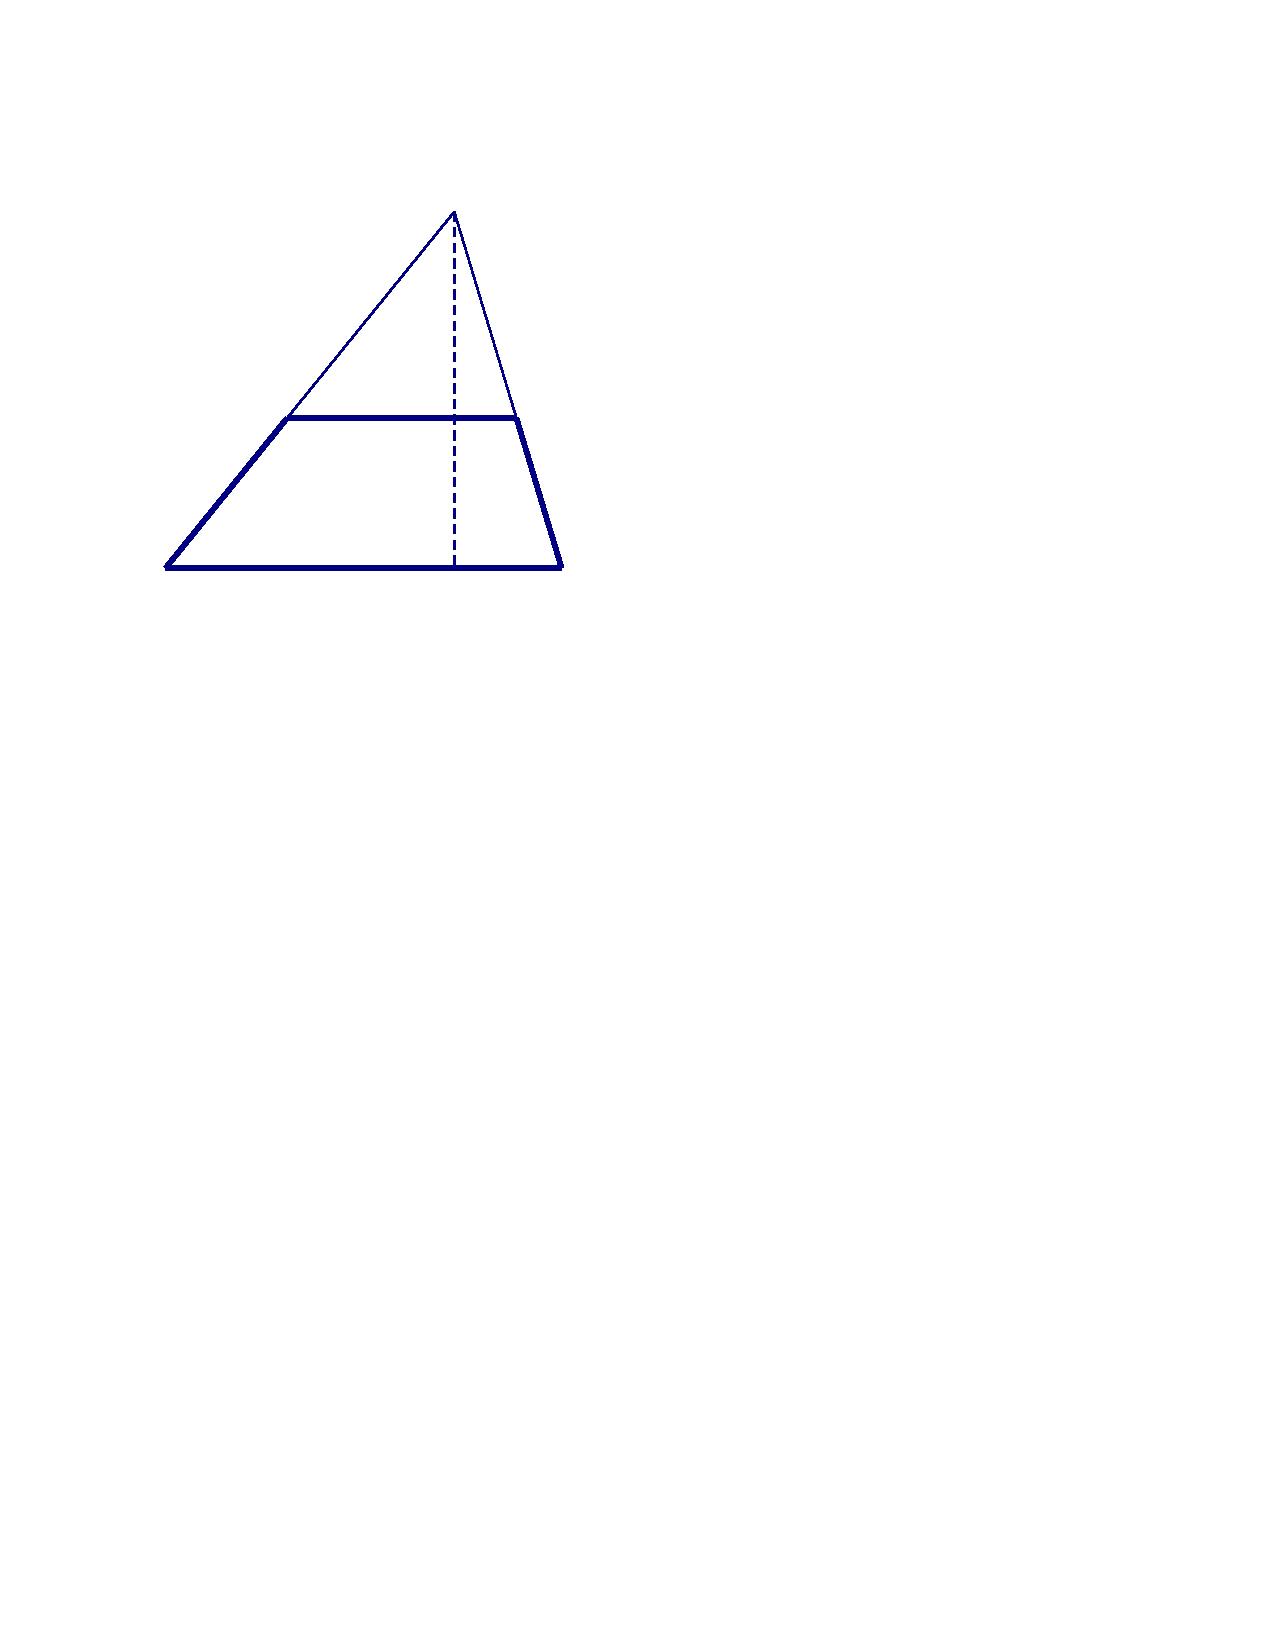
\includegraphics[scale=0.7]{../graphics/trapezoid6.pdf}&  \hspace{\formulawidth} \\ \hline
\end{tabular}}

%%
%%   Answers
%%
\begin{teachingnote}
\newpage
{\renewcommand{\arraystretch}{1.5}
\begin{tabular}{|>{\centering\arraybackslash}m{2.5cm}|>{\centering\arraybackslash}m{9.5cm}|c|}\hline
Explanation & Figure & Area Formula \\\hline

Rectangle with width that is the average of the bases. & 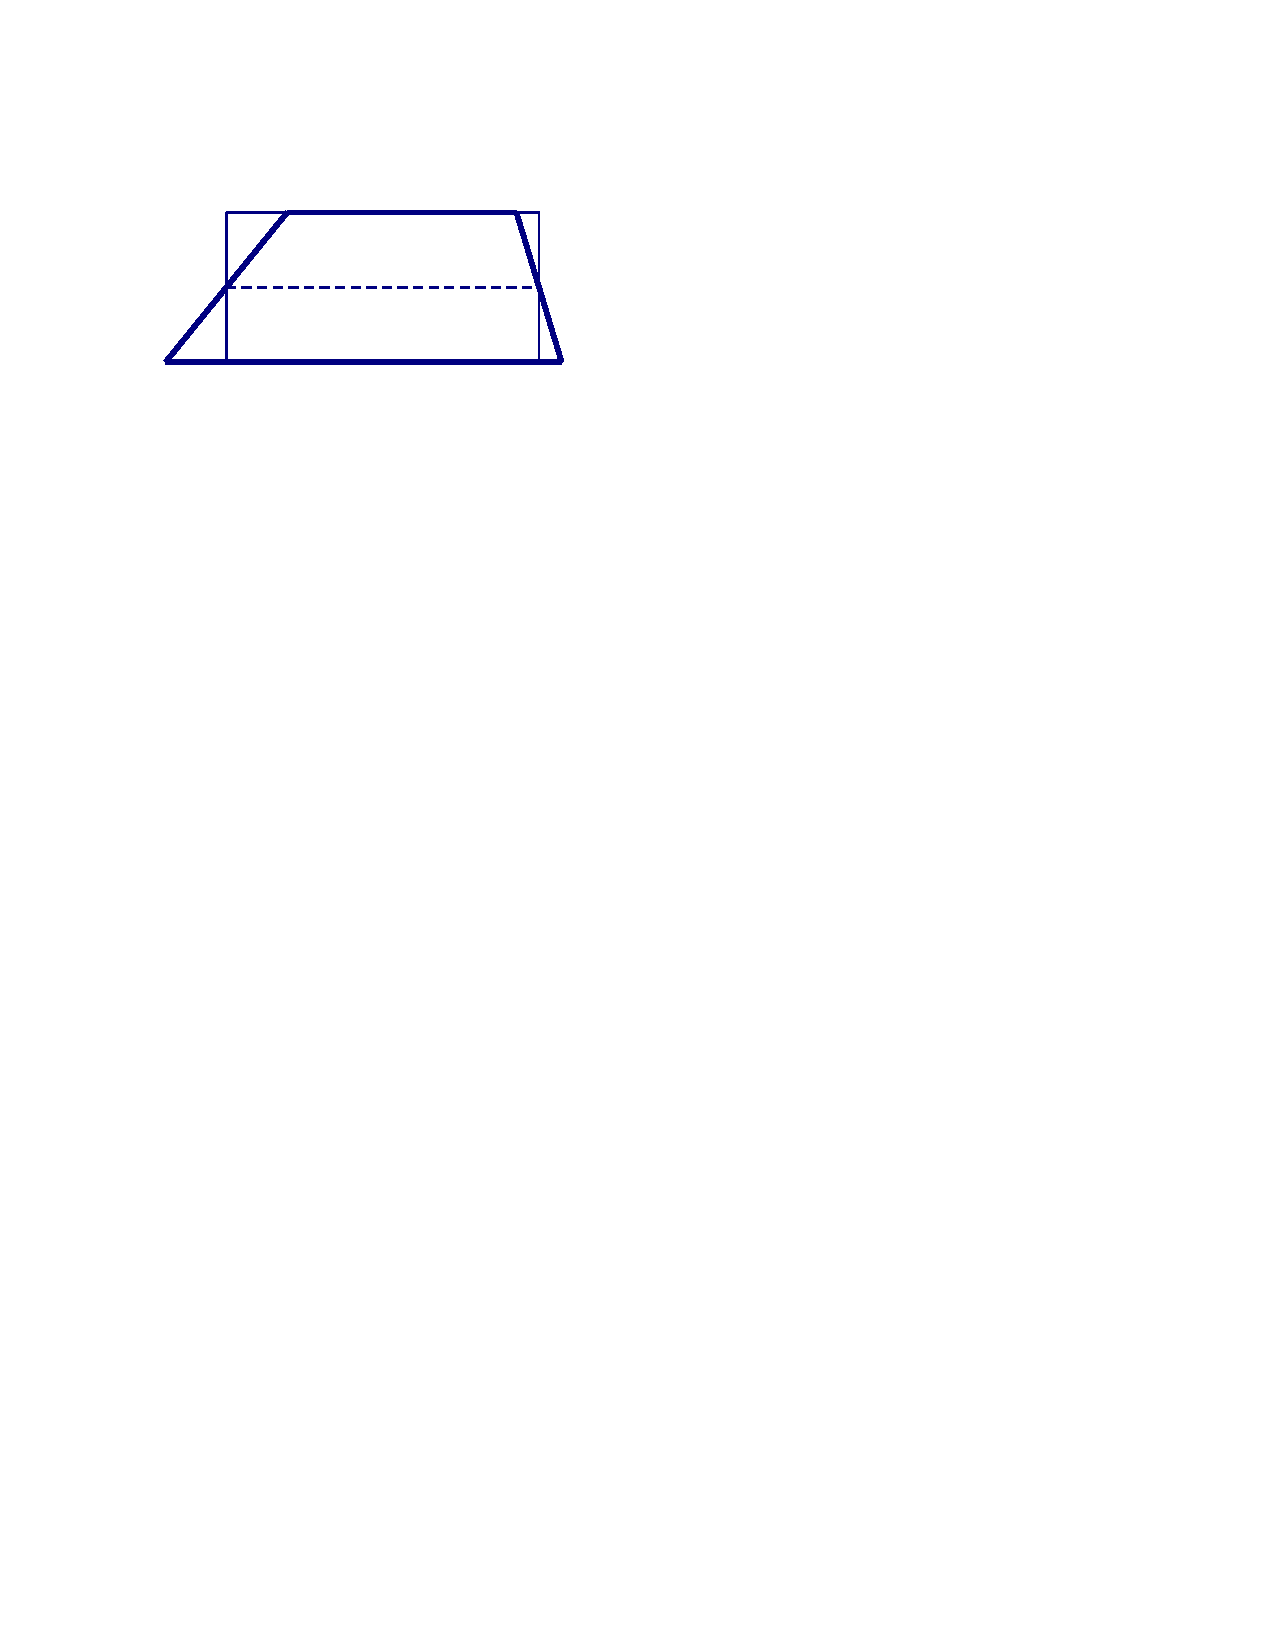
\includegraphics[scale=0.7]{../graphics/trapezoid2.pdf} & $\left(\frac{b_1+b_2}{2}\right)h$ \\ \hline
Half of a large parallelogram. & 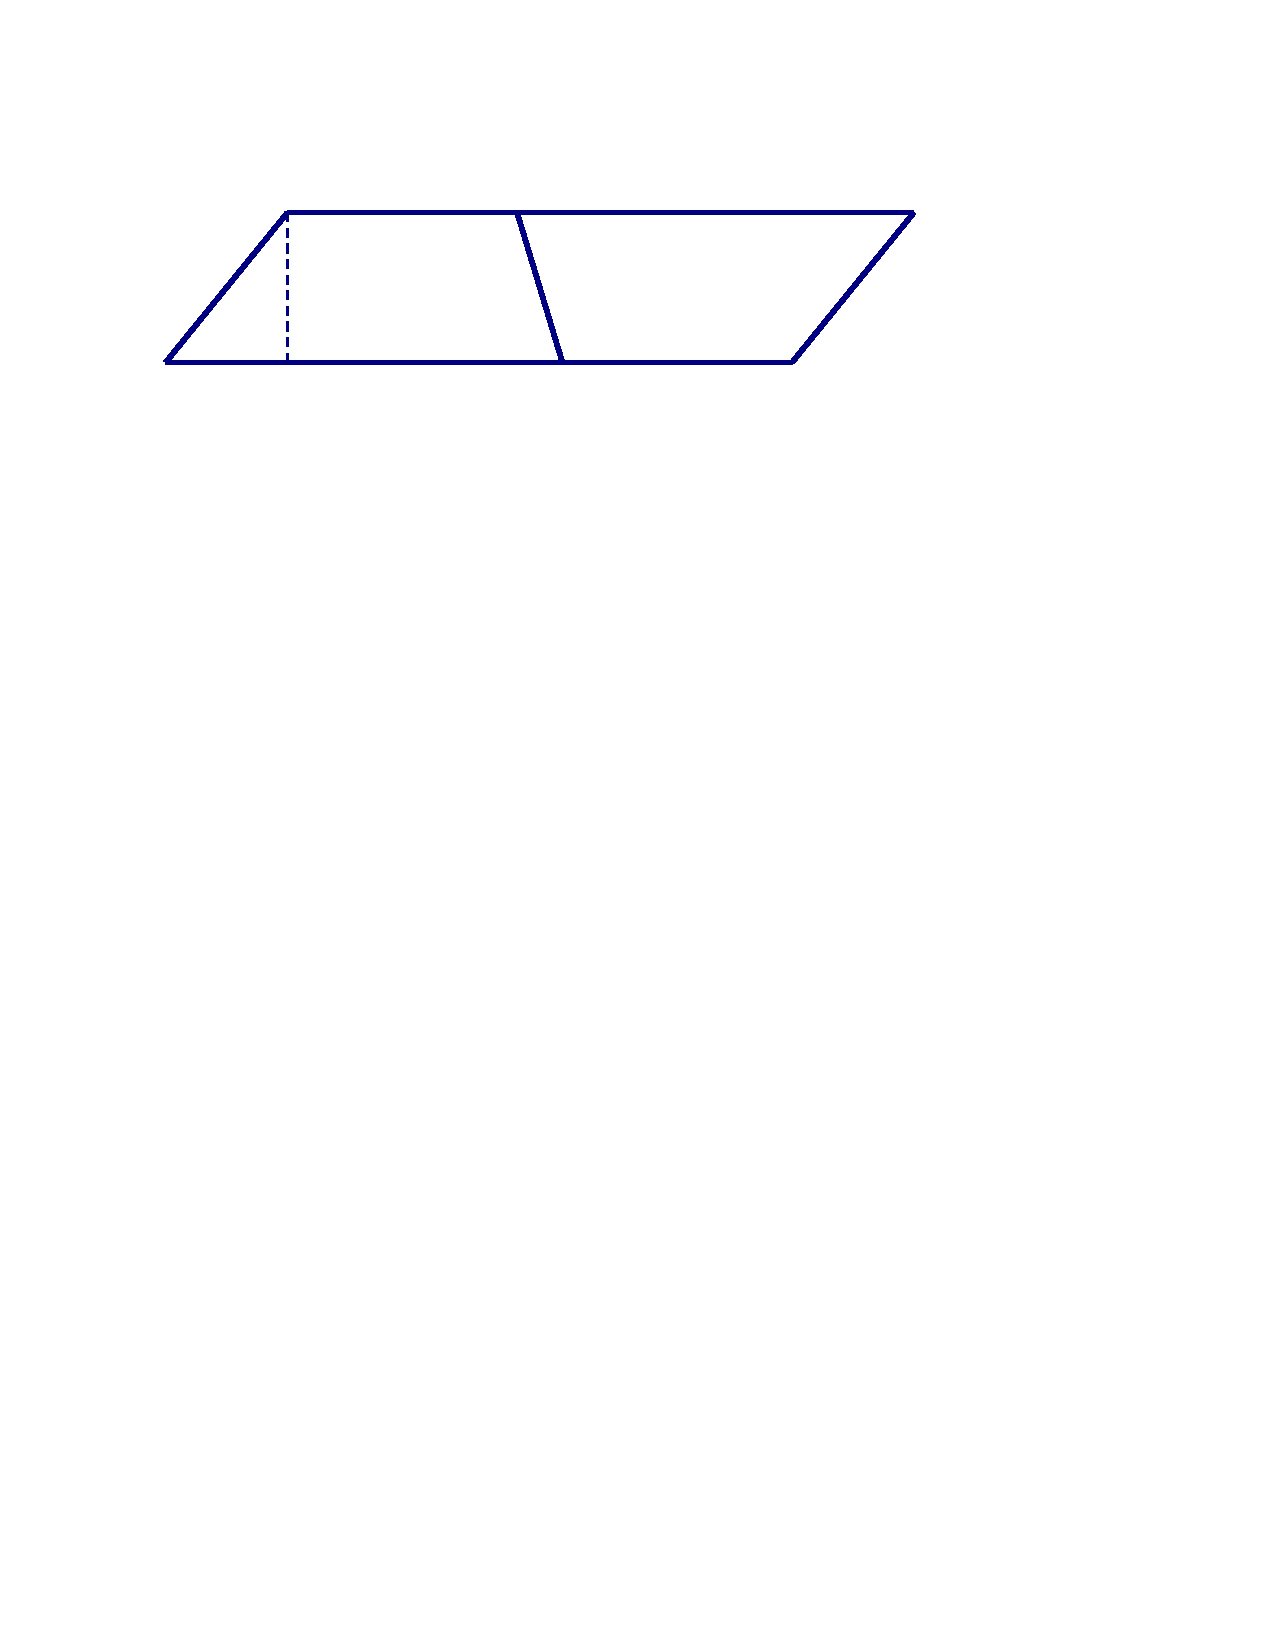
\includegraphics[scale=0.7]{../graphics/trapezoid3.pdf} & $\frac{1}{2}(b_1+b_2)h$ \\ \hline
Two triangles with the same height and different bases. & 
\includegraphics[scale=0.7]{../graphics/trapezoid4.pdf} & $\frac{1}{2}b_1h + \frac{1}{2}b_2h$ \\ \hline
A parallelogram with half the height. & 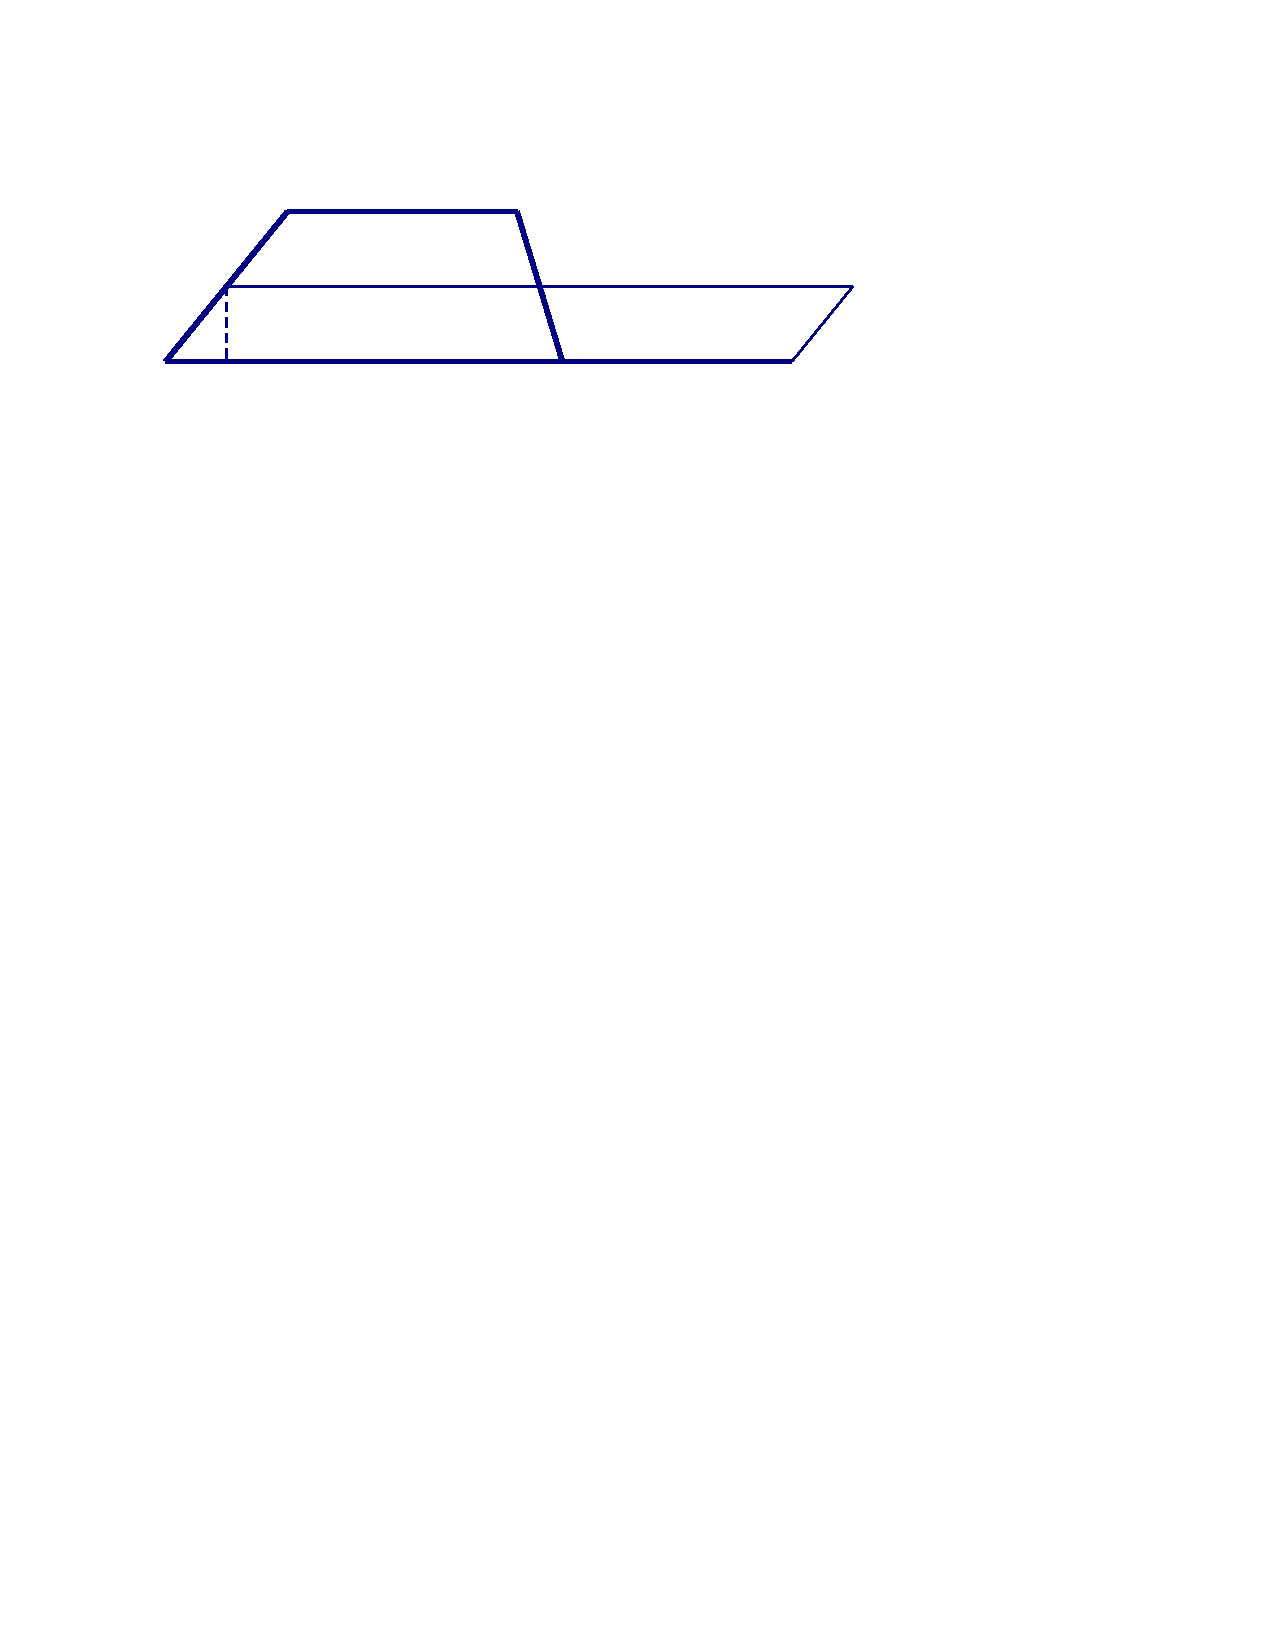
\includegraphics[scale=0.7]{../graphics/trapezoid5.pdf} & $(b_1+b_2)\frac{h}{2}$ \\ \hline
Difference between two triangles, with $x$ as height of small triangle. 
          & 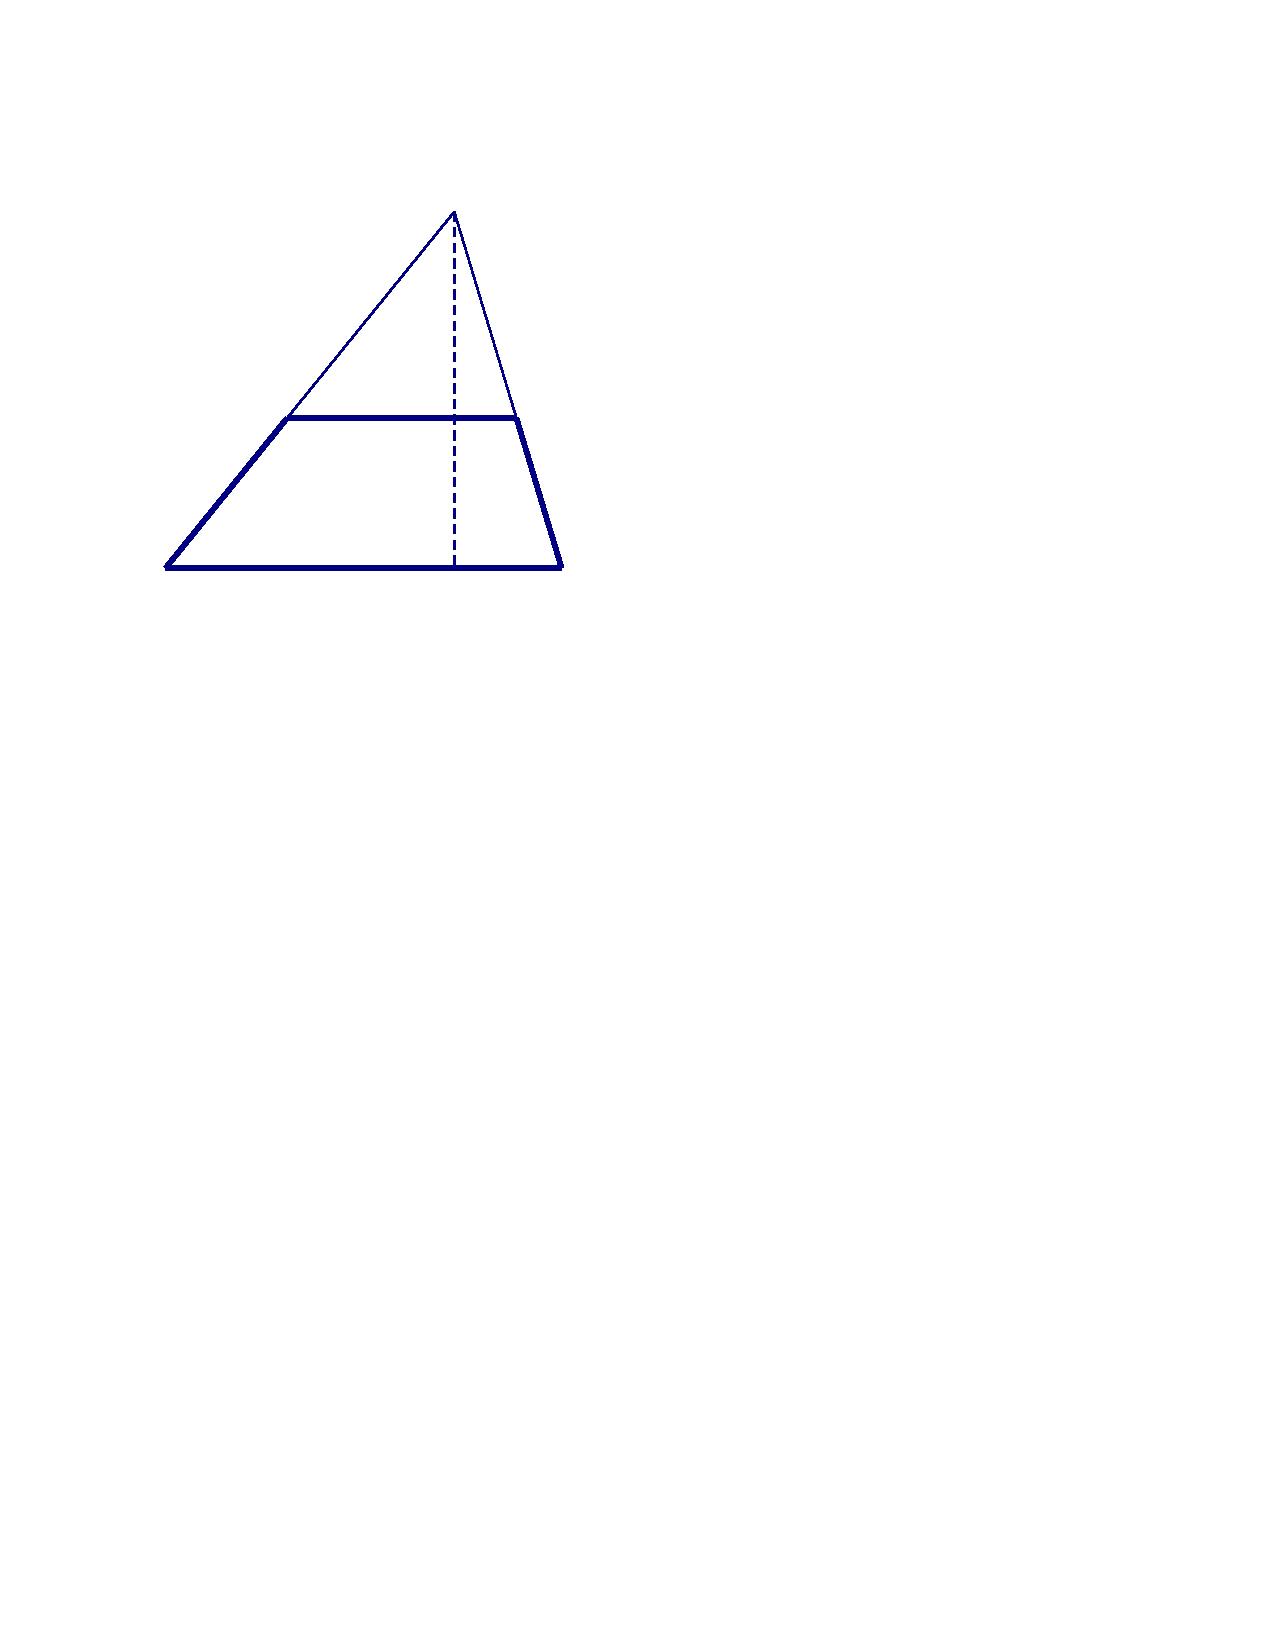
\includegraphics[scale=0.7]{../graphics/trapezoid6.pdf} &  $\frac{1}{2}b_2(x+h)-\frac{1}{2}b_1x$, with $\frac{x}{b_1}=\frac{x+h}{b_2}$ \\ \hline
\end{tabular}}
\end{teachingnote}

\end{prob}
